\chapter{Resultados} \label {chap:resultados}
	\section{Introducción} 
	
	Este capítulo presenta los resultados obtenidos durante la implementación de cada uno de los prototipos planteados en el Capítulo
	~\ref{chap:disenoeimpl} y durante la ejección de los casos de prueba correspondientes. 
\begin{itemize}
\item Se instanciaron los proyectos MinSoC y ORPSoC, ambos con núcleo OpenRISC. 
\item Se evaluó el funcionamiento del microprocesador OpenRISC con programa de prueba de multiplicación de matrices binarias cuadradas.
\item Se evaluaron las capacidades del compilador cruzado or32-elf-gcc en lo referido a su capacidad de optimización de código. 
\item Se ejecutaron los benchmarks de sistemas embebidos \verb|coremark| y \verb|dhrystone| para posicionar el microprocesador OpenRISC entre CPUs de similares
características.
\item Se realizó la implementación de dos sistemas operativos, uno de tiempo real (ecOS) y uno de mayores capacidades (Linux). 
\end{itemize}				
				
	Para la ejecución de todas las pruebas se utilizó la placa desarrollo S3ADSP1800A del fabricante Xilinx que cumple con los requerimientos detallados
	en la tabla~\ref{tab:requsr1} y se encontraba dentro de las alternativas disponibles al momento del desarrollo de este trabajo. Durante el desarrollo de las pruebas se pretendió establecer los límites de aplicación del proyecto
	que establezcan referencias sólidas para una futura elección del proyecto en aplicaciones reales.


	\newpage
	\section{Resultados de Utilización de FPGA en la Implementación del Proyecto MinSoC}

El proyecto MinSoC se encuentra enfocado a su utilización en sistemas embebidos de capacidades ajustadas sintetizables en una gran cantidad de FPGA de diversos desarrolladores. En la tabla ~\ref{tab:conbench} se presentan con éxito la implemantación del proyecto en uno de los kit de desarrollo soportado por el proyecto y disponible para su uso en el laboratorio CUDAR.

\begin{table}[h!]
		\begin{tabular}{ |p{6cm} |p{3cm} |p{3cm}| p{3cm}| }    
		\hline
		\multicolumn{4}{|>{\columncolor[gray]{.8}}c}{Resumen de utilización MinSoC}\\
		\hline
		\multicolumn{1}{|>{\columncolor[gray]{.8}}c}{Logica utilizada} & \multicolumn{1}{|>{\columncolor[gray]{.8}}c}{Usado} & \multicolumn{1}{|>{\columncolor[gray]{.8}}c}{Disponible} & \multicolumn{1}{|>{\columncolor[gray]{.8}}c}{Utilizado} \\
		\hline 
		Slice Flip Flop & 5040 & 33280 & 15\%  \\ 
		\hline 
		LUTs de 4 entradas & 13901 & 33280 & 41\%  \\ 
		\hline 
\multicolumn{1}{|>{\columncolor[gray]{.8}}c}{Logica de distribución} & \multicolumn{1}{|>{\columncolor[gray]{.8}}c}{Usado} & \multicolumn{1}{|>{\columncolor[gray]{.8}}c}{Disponible} & \multicolumn{1}{|>{\columncolor[gray]{.8}}c}{Utilizado} \\
		\hline 
		Slice & 8475 & 16640 & 50\%  \\ 
		\hline 
		Luts de 4 entradas para lógica combinacional& 13866 & 33280 & 40\%  \\ 
		\hline 
		Luts de 4 entradas route-thru & 330 & 33280 & 1\%  \\ 		
		\hline 
		Luts de 4 entradas para puertos Dual RAM & 32 & 33280 & 0,9\%  \\ 		
		\hline 
		Luts de 4 entradas para shift registers & 3 & 33280 & 0,1\%  \\ 
		\hline
		IOBs& 29 & 519 & 5\%  \\ 
		\hline 
		BUFGMUXs & 5 & 24 & 20\%  \\ 
		\hline 
		DCMs & 1 & 8 & 12\%  \\ 
		\hline
		DSP48As & 4 & 84 & 4\%  \\ 
		\hline 
		RAMB16BWERs & 70 & 84 & 83\%  \\ 
		\hline 
		BSCAN\_SPARTAN3As& 1 & 1 & 100\%  \\ 
		\hline 
\end{tabular}
%\end{center}
\caption{Resultados de la implementación del proyecto MinSoC}
\label{tab:conbench}
\end{table}

Como se puede observar los resultados obtenidos luego del proceso completo de implementación del proyecto MinSoC, desde el punto de vista de utilización lógica se utilizó el 15\% de Slice Flip Flops y el 41\% de LUTs disponibles en la FPGA.  Respecto de la distribución lógica se tiene un 50\% de ocupación de Slices y un 42\% de LUTs de 4 entradas de las cuales el 1\% se utiliza
	como LUTs de paso o en inglés route-thru. El 41\% restante están utilizadas como lógica combinacional , puertos Dual RAM y registros de
	desplazamiento. Se utilizó el 5\% de los bloques de entrada/salida, el 20\% de los BUFGMUXs ó buffers de clock global, el 12\% de los DCMs, el 4\% de
	los bloques DSP y el 83\% de los bloques de RAM. El proceso Technology Mapping utilizó un pico 415 MB de memoria.

Teniendo en cuenta los datos obtenidos y la facilidad de adaptación del proyecto para portarse a otras arquitecturas reconfigurables, se pueden aproximar los límites de la aplicación del proyecto para el uso mas eficiente de los recursos provistos de una futura elección en placas de desarrollo, derivando esto, por ejemplo en reducción de costos.


\newpage
	\section{Resultados de Utilización de FPGA en la Implementación del Proyecto ORPSoC}

El proyecto ORPSoC también se encuentra enfocado a su utilización en sistemas embebidos de capacidades ajustadas sintetizables en una gran cantidad de FPGA de diversos desarrolladores. A continuación en la tabla~\ref{tab:conbench1} se presentan con éxito la  implementación del proyecto sobre el kit de desarrollo de Xilinx.
		
\begin{table}[h!]
		\begin{tabular}{ |p{6cm} |p{3cm} |p{3cm}| p{3cm}| }    
		\hline
		\multicolumn{4}{|>{\columncolor[gray]{.8}}c}{Resumen de utilización ORPSoC}\\
		\hline
		\multicolumn{1}{|>{\columncolor[gray]{.8}}c}{Logica utilizada} & \multicolumn{1}{|>{\columncolor[gray]{.8}}c}{Usado} & \multicolumn{1}{|>{\columncolor[gray]{.8}}c}{Disponible} & \multicolumn{1}{|>{\columncolor[gray]{.8}}c}{Utilizado} \\
		\hline 
		Slice Flip Flop & 4872 & 33280 & 14\%  \\ 
		\hline 
		LUTs de 4 entradas & 12093 & 33280 & 36\%  \\ 
		\hline 
\multicolumn{1}{|>{\columncolor[gray]{.8}}c}{Logica de distribución} & \multicolumn{1}{|>{\columncolor[gray]{.8}}c}{Usado} & \multicolumn{1}{|>{\columncolor[gray]{.8}}c}{Disponible} & \multicolumn{1}{|>{\columncolor[gray]{.8}}c}{Utilizado} \\
		\hline 
		Slice &7772 & 16640 & 46\%  \\ 
		\hline 
		Luts de 4 entradas para lógica combinacional& 11009 & 33280 & 33\%  \\ 
		\hline 
		Luts de 4 entradas route-thru & 250 & 33280 & 0,7\%  \\ 		
		\hline 
		Luts de 4 entradas para puertos Dual RAM & 960 & 33280 & 3\%  \\ 		
		\hline 
		Luts de 4 entradas para Shift registers & 124 & 33280 & 0,3\%  \\ 
		\hline 		
		IOBs& 128 & 519 & 24\%  \\ 
		\hline  
		BUFGMUXs & 7 & 24 & 29\%  \\ 
		\hline 
		DCMs & 2 & 8 & 25\%  \\ 
		\hline
		DSP48As & 4 & 84 & 4\%  \\ 
		\hline 
		RAMB16BWERs & 16 & 84 & 19\%  \\ 
		\hline 
		BSCAN\_SPARTAN3As& 1 & 1 & 100\%  \\ 
		\hline 
\end{tabular}
%\end{center}
\caption{Resultados de la implementación del proyecto ORPSoC}
\label{tab:conbench1}
\end{table}	
		
	Como se puede observar que desde el punto de vista de utilización lógica se utilizó el 14\% de Slice Flip Flops y el 36\% de LUTs disponibles en
	la FPGA. Respecto de la distribución lógica se tiene un 46\% de ocupación de Slices y un 37\% de LUTs de 4 entradas de las cuales el 0,7\% se utiliza
	como LUTs de paso o en inglés route-thru. El 36\% restante están utilizadas como lógica combinacional , puertos Dual RAM y registros de
	desplazamiento. Se utilizó el 24\% de los bloques de entrada/salida, el 29\% de los BUFGMUXs ó buffers de clock global, el 25\% de los DCMs, el 4\%
	de los bloques DSP y el 19\% de los bloques de RAM. El proceso Technology Mapping utilizó un pico 410 MB de memoria.  
 
Al igual que en la implemetación del proyecto anterior en la placa de desarrollo de Xilinx,  teniendo en cuenta la capacidad de adaptación a otras arquitecturas reconfigurable que tiene el proyecto ORPSoC, con los datos obtenidos se llego a la conclusión de que seria viable implemtarlo en placas mas pequeñas y de menor costo.

%		\subsection{Reporte de timing}	
%
%El reporte de timing presenta los resultados del análisis de distribución de los clocks del proyecto. Entre los resultados se obtiene el mínimo
%periodo (Máx Frecuencia) necesarios para el correcto funcionamiento del sistema. Es importante destacar que los tiempos expuestos en el reporte son
%teóricos y se presentan cambios importante durante las pruebas sobre el hardware. 
%
%\begin{lstlisting}[frame=single,caption={Reporte timing - ORPSoC},label={lst:salidas},breaklines]
%Timing summary:
%
%Timing errors: 498  Score: 729028  (Setup/Max: 311057, Hold: 417971)
%Constraints cover 395663179 paths, 94 nets, and 53193 connections
%
%Design statistics:
%  Minimum period:  45.166ns   (Maximum frequency:  22.141MHz)
%  Maximum path delay from/to any node:  11.696ns
%  Maximum net delay:   2.594ns
%  Minimum input required time before clock:  26.237ns
%  Maximum output delay after clock:  13.126ns
%\end{lstlisting}



\newpage
\section {Estudio de Capacidades del Proyecto MinSoC}
		
		\subsection{Estudio de la complejidad del algoritmo de prueba}
		
		El tiempo de ejecución de un algoritmo va a depender de diversos factores como son: los datos de entrada que le suministremos, la calidad del
		código generado por el compilador para crear el programa objeto, la naturaleza y rapidez  de las instrucciones máquina del procesador concreto que
		ejecute el programa, y la complejidad intrínseca del algoritmo. Hay dos estudios posibles sobre el tiempo: 
 
		\begin{itemize}
		  \item Uno que proporciona una medida teórica (a priori), que consiste en obtener una  función que acote (por arriba o por abajo) el tiempo de
		  ejecución del algoritmo para unos valores de entrada dados.
		\item Y otro que ofrece una medida real (a posteriori), consistente en medir el tiempo  de ejecución del algoritmo para unos valores de entrada
		dados y en un ordenador concreto. 
		\end{itemize} 
		
		Entendemos por tamaño de la entrada el número de componentes sobre los que  se va a ejecutar el algoritmo. Por ejemplo, la dimensión del vector a
		ordenar o el tamaño de las matrices a multiplicar. La unidad de tiempo a la que debe hacer referencia estas medidas de eficiencia  no puede 
		expresarse en segundos o en otra unidad de tiempo concreta, pues no existe un ordenador estándar al que puedan hacer referencia todas las medidas. 
        Denotaremos por T(n) el tiempo de ejecución de un algoritmo para una entrada de tamaño n. 
        
        También es importante hacer notar que el comportamiento de un algoritmo puede cambiar notablemente para diferentes entradas (por ejemplo, los
        ordenados que se encuentren ya los datos a ordenar). De hecho, para muchos programas el tiempo de ejecución es en realidad una función de la
        entrada específica, y no sólo del tamaño de ésta. Así suelen estudiarse tres casos para un mismo algoritmo: caso peor, caso mejor y caso
        medio. El caso mejor corresponde a la traza (secuencia de sentencias) del algoritmo que realiza menos instrucciones. Análogamente, el caso
        peor corresponde a la traza del algoritmo que realiza más instrucciones.
 		
 		A la hora de medir el tiempo, siempre lo haremos en función del número de operaciones elementales que realiza dicho algoritmo, entendiendo por
 		operaciones elementales (en adelante OE) aquellas que el ordenador realiza en tiempo acotado por una constante. Así, consideraremos OE las
 		operaciones aritméticas básicas,  asignaciones a variables de tipo predefinido por el compilador, los saltos (llamadas a funciones y
 		procedimientos, retorno desde ellos, etc.), las comparaciones lógicas y el acceso a estructuras indexadas básicas, como son los vectores y
 		matrices. Cada una de ellas contabilizará como 1 OE. Resumiendo, el tiempo de ejecución de un algoritmo va a ser una función que mide el número de
 		operaciones elementales que realiza el algoritmo para un tamaño de entrada dado.
		
		Se define a continuación la complejidad de cálculo para el multiplicador de matrices binarias implementado en la sección ~\ref {testing:proto1} que
		cuenta con tres bucles anidados y operaciones de multiplicación y acumulación.
	
\newpage			
	\begin{lstlisting}[language=C,frame=single , caption={Código del programa de prueba multiplicador de matrices binarias}]
for (i=0;i<indice;i++){						(*1*)
  for (j=0;j<indice;j++){					(*2*)
    for (k=0;k<indice;k++){					(*3*)
	  producto = matrizA[i*con+k] * matrizB[k*con+j];	(*4*)
	  acumulador = acumulador + producto;			(*5*) 
    }								(*6*)
  matriz [i*con+j] = acumulador;				(*7*)
  acumulador = 0;						(*8*)
  }								(*9*)
}								(*10*)
	\end{lstlisting}
		
	    Para determinar el tiempo de ejecución, calcularemos primero el número de operaciones elementales (OE) que se realizan: 
 		\begin{itemize}
 		  \item En la línea (1) En la primera iteración del bucle si tiene una asignación. Luego se efectúa la condición del bucle que depende de ``i'' con
 		  una comparación y un post incremento de i. (2 OE)
 		  \item En la línea (2) En la primera iteración del bucle si tiene una asignación. Se efectúa la condición del bucle que depende de ``j'' con una
 		  comparación y un post incremento de j. (2 OE)
 		  \item En la línea (3) En la primera iteración del bucle si tiene una asignación. Se efectúa la condición del bucle que depende de ``k'' con una
 		  comparación y un post incremento de k. (2 OE)
 		  \item La línea (4) está compuesta por una asignación, dos accesos a vectores, dos incrementos y tres productos. (8 OE) 
 		  \item La línea (5) está compuesta por una asignación y una suma (2 OE)
 		  \item En la línea (6) se tiene fin del bucle que depende de ``k'' (1 OE)
 		  \item En la línea (7) se tiene una asignación , un incremento, un producto y un acceso a vector (4 OE)
 		  \item En la línea (8) se tiene una asignación (1 OE)
 		  \item En la línea (9) se tiene fin del bucle que depende de ``j'' (1 OE)
 		  \item En la línea (10) se tiene fin del bucle que depende de ``i'' (1 OE)
 		\end{itemize}
		
		Se establece que indice = n (todas matrices cuadradas nxn). Se tiene entonces: 
		
		\begin{equation*}
		T(n) = 1 + \sum_{i=0}^{n-1} \left (2 + \sum_{j=0}^{n-1} \left (2 + \sum_{k=0}^{n-1} 1 + (8+2)\right ) + (4 + 1) \right )      
		\end{equation*}
		
		Obteniendo de esta manera:
		
		\begin{equation*}
		T(n) = 11 n^3 + 9 n^2 + 1       
		\end{equation*}
		 
		
		\subsection{Resultados de la ejecución del multiplicador de matrices binarias}
			
		Se presentan a continuación los resultados de ejecución del programa multiplicador de matrices binarias. Se utilizó un gráfico que muestra el orden
		de las matrices multiplicadas vs. la cantidad de ticks de ejecución. El figura~\ref{fig:mulmat} muestra con claridad que el tiempo de ejecución
		aumenta exponencialmente a medida que aumenta el orden de las matrices multiplicadas.
		
\begin{figure}[h!]
 	\begin{center}
  	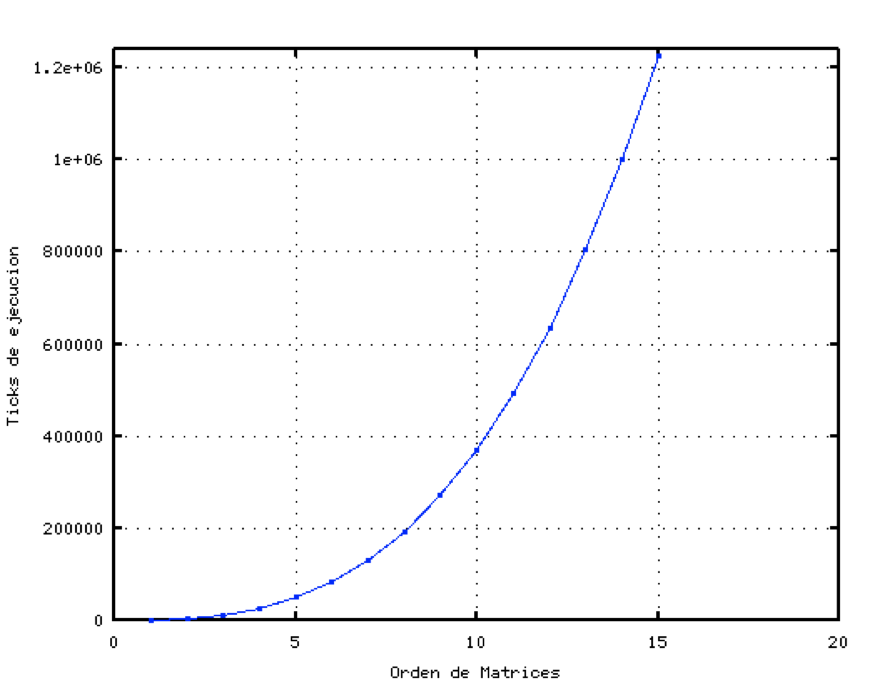
\includegraphics[width=0.9\textwidth,keepaspectratio=true]{./images/calculomatriz}
  	\caption{Multiplicación de matrices binarias}
  	\label{fig:mulmat}
 	\end{center}
	\end{figure}

		Teniendo en cuenta que la aplicación ejecutó en una versión sintentizada básica del proyecto minSoC, este no posee unidades de multiplicación
		por hardware que efectuen cálculos con mayor eficiencia, reduciendo el tiempo de ejecución. Pueden considerarse también, las optimizaciones del
		compilador, pero este aspecto fue analizado en el Prototipo Tres con mayor detalle. 	

        \subsection{Estudio de los niveles y banderas de optimización del compilador cruzado}
		\subsubsection{Optimización de código}
		
El objetivo de la optimización de código por parte del compilador es obtener código que se ejecuta más eficientemente según los criterios:
\begin{itemize}
  \item Tiempo de ejecución (optimización temporal)
  \item Espacio de memoria utilizado (optimización espacial) 
\end{itemize}
 
El funcionamiento básico de este mecanismo consiste en que el compilador revisa el código generado a varios niveles de abstracción y realiza las
optimizaciones aplicables al nivel de abstracción.
\begin{itemize}
  	\item Árbol sintáctico abstracto: optimizar subexpresiones redundantes, reducción de frecuencia, etc.
	\item Tuplas o cuadruplas: optimizar el uso de los registros o de las variables temporales.
	\item Ensamblador/Código máquina: convertir saltos a saltos cortos, reordenar instrucciones
\end{itemize}

Se define un bloque básico como un fragmento de código que tiene una única entrada y salida, y cuyas instrucciones se ejecutan secuencialmente. Si se
ejecuta una instrucción del bloque se ejecutan todas en un orden conocido en tiempo de compilación. La idea del bloque básico es encontrar partes del programa
cuyo análisis necesario para la optimización sea lo más simple posible.

Una técnica bien conocida para la optimización de bucles es la llamada desenrrolado de bucles (Loop Unrolling). La expansión de bucles solo se puede
aplicar a los bucles cuyo número de iteraciones se conoce en tiempo de compilación. La expansión de un bucle puede ser muy costosa en espacio. Hay
que poner un criterio heurístico para decidir si se aplica la expansión. Se puede aplicar una expansión parcial en la que sigue existiendo el bucle,
pero cada iteración del nuevo bucle corresponde a varias iteraciones del bucle original. En un bucle expandido se ha de sustituir el índice del bucle 
por el valor constante correspondiente.

El compilador cruzado utilizado en este trabajo or32-elf-gcc Versión 4.5.1 permite realizar optimizaciones de código mediante una serie de flags que
identifican cada uno de los mecanismos de optimización que el compilador implementa. Los flags fueron utilizados durante la ejecución de pruebas en
este trabajo son:

\begin{itemize}
  	\item -O2 : Este nivel de optimización activa una serie de flags que pueden consultarse en \cite{etiqueta_OptGcc}
	\item -O3 : Este nivel de procura una mayor optimización de código y activa una serie de flags conjunto con los del nivel -O2 que pueden consultarse
	en \cite{etiqueta_OptGcc}
	\item -funroll-loops : Desenrrolla los bucles cuyo número de iteraciones puede ser determinado en tiempo de compilación. 
	\item -funroll-all-loops : Desentrolla todos los bucles aún cuando el número de iteraciones no pueda determinarse en tiempo de compilación. 
	\item -fgcse-sm : Cuando este flag se encuentra activado, el compilador procura mover fuera de los bucles las operaciones store.
\end{itemize}

		\subsubsection{Resultados de la compilación de un bucle simple}

A modo de prueba se planteó un programa que incluye un arreglo de elementos enteros y dos bucles ``for'' , uno para la inicialización del arreglo y
otro para su actualización.

	\begin{lstlisting}[language=C,frame=single , caption={Código del programa de prueba de opciones de optimización del compilador (bucle simple) }]
#define ITERACIONES 1000
#define CTE 3

int x [ITERACIONES];
int i ;

void set (){
	for (i=0;i<ITERACIONES;i++)
		x[i] = 4;
}

void calc () {
	for (i=0;i<ITERACIONES;i++)
		x[i] = x[i] + CTE;
}

void main () {
	set ();
	calc ();
}
	\end{lstlisting}
		
En una primera instancia se realizó el desensamblado del binario generado para las funciones set (inicialización) y calc (actualización) con un
numero de 1000 iteraciones y para cada uno de los flags de optimización. Los códigos generados pueden observarse en detalle en el apéndice~\ref{chap:CodPrueba}. 
\newpage		
A continuación se presenta en la tabla~\ref{tab:conbench2} el resume de los resultados obtenidos para 1000 iteraciones y diversos flags de optimización:

\begin{table}[!h]
		\centering
		\begin{tabular}{ | p{4cm} | p{5cm} | p{2.5cm} | p{2cm} | }
		\hline 
		\rowcolor[gray]{0.8} Función & Flags & Cantidad de Instrucciones  & Registros Utilizados \\    
		\hline 
		set (inicialización) 	& -O2 						& 19 &  4 \\ 
		\hline 
							 	& -O2 -funroll-loops 		& 25 &  7 \\ 
		\hline 
							 	& -O2 -funroll-all-loops 	& 25 &  7 \\ 
		\hline 
							 	& -O3 						& 19 &  4 \\ 
		\hline 
							 	& -O3 -funroll-loops 		& 25 &  7 \\ 
		\hline 
							 	& -O3 -funroll-all-loops 	& 25 &  7 \\ 
		\hline 
		calc (actualización) 	& -O2						& 19 &  4 \\ 
		\hline 
							 	& -O2 -funroll-loops 		& 47 &  20 \\ 
		\hline 
							 	& -O2 -funroll-all-loops 	& 47 &  20 \\ 		
		\hline					 	
							 	& -O3 						& 19 &  4 \\ 
		\hline 
							 	& -O3 -funroll-loops 		& 47 &  20 \\ 
		\hline 
							 	& -O3 -funroll-all-loops 	& 47 &  20 \\ 		
		\hline 
		\end{tabular}
\caption{Resultados de la compilación del programa de prueba con diversos flags de optimización}
\label{tab:conbench2}
\end{table}	

%\newpage		

\section {Estudio de Capacidades del Proyecto ORPSoC}	
		\subsection{Condiciones de entorno de ejecución para benchmark}
		
		En la siguente tabla~\ref{tab:conbench} se muestran las condiciones del entorno de prueba durante los benchmarks.  

		\begin{table}[h!]
		\begin{tabular}{ |p{5cm} |p{10cm}| }    
		\hline
		\multicolumn{2}{|>{\columncolor[gray]{.8}}c}{Condiciónes de entorno de prueba|}\\
		\hline
		Placa de desarrollo & S3ADSP1800A  \\
		\hline 
		FPGA & Xilinx Spartan-3 XC3SD1800A \\ 
		\hline 
		Reloj del procesador & 25 MHz\\ 
		\hline
		Caché de instrucciones  & 8 KB \\ 
		\hline
		Caché de datos	  & 8 KB\\ 
		\hline	
		MMU & Sí \\	
		\hline
		Multiplicador hardware & Sí \\		
		\hline	
		División hardware & Sí \\		
		\hline	
		Punto Flotante & Precisión simple \\		
		\hline
\end{tabular}
%\end{center}
\caption{Condiciones del entorno de prueba}
\label{tab:conbench}
\end{table}


		\subsection{Resultados de la ejecución del benchmark CoreMark}
		
Inicialmente se prensentan los valores obtenidos durante la ejecución del Benchmark compilado con optimizaciones de nivel 2 (-O2) del
compilador cruzado. El Benchmark CoreMark arroja un valor de  41.288895/25MHz = 1.65/MHz como resultado de la prueba. Las condiciones de ensayo se
detallan en la tabla~\ref{tab:conbench} y la ejecución se realizó con 600 iteraciones. 


%	\subsection {Presentación de los resultados de optimización} 

En la tabla~\ref{tab:conbench2} se presentan los resultados de ejecutar el CoreMark en la placa de desarrollo de Xilinx, obtenidos mediante la utilización de optimización en la fase de compilación. Sin ningún tipo de optimización el valor del CoreMark fue 0,49/MHz.

\begin{table}[!h]
\begin{center}
\begin{tabular}{ |l |c |c |c |c|}
\hline
\rowcolor[gray]{0.8} Opciones del compilador&-O2& Optimización &-O3& Optimización \\
\hline
Sin extras 					& 1.41 	& 			& 1.45 &  \\
\hline
-mhard-div -mhard-mu 		& 1.41	& 0\%		& 1.45 & 0\% \\
\hline
-funroll-loops			 	& 1.53	& 8\%		& 1.50 & 4\%\\
\hline
-fgcse-sm					& 1.42	& 0,7\%		& 1.46 & 0,6\%\\
\hline
-msoft-float 				& 1.41	& 0\%		& 1.45 & 0\%\\
\hline
-funroll-all-loops	 		& 1.55	& 10\%		& 1.52 & 5\%\\
\hline
Todos	 					& 1.55	& 10\%		& 1.52 & 5\%\\
\hline
\end{tabular}
\end{center}
\caption{Compilación con distintos niveles y flags de optimización}
\label{tab:conbench2}
\end{table}

Se puede observar que se mejoró el valor del CoreMark para un nivel de optimizacion -O2 en un 65\% y para un nivel de optimización -O3 en un 66\% con respecto al valor sin ningún tipo de optimización. Luego agregando flags a cada nivel de compilación se pudo obtener para un nivel de optimización -O2 una mejora del 10\% y para un nivel de optimización -O3 una mejora del 5\%  con respecto el valor obtenido sin ningún flag habilitado en cada nivel de optimización. 


%  A continuación se muestran en el bloque ~\ref{lst:salidasO2} algunas de las salidas que resultan de ejecutar el CoreMark compilado con el nivel de optimización -O2, -O3 y diferentes flags de optimización se observaron los resultados mostrados en el bloque ~\ref{lst:salidasO2}
% 
% \begin{lstlisting}[frame=single,caption={Optimización nivel -O2 - Flags activos : -FUNROLL-LOOPS },label={lst:salidasO2},breaklines]
% 2K validation run parameters for coremark.
% CoreMark Size    : 666
% Total ticks      : 1527
% Total time (secs): 15.270000
% Iterations/Sec   : 39.292731
% Iterations       : 600
% Compiler version : GCC4.5.1-or32-1.0rc4
% Compiler flags   : -O2  -mboard=s3adsp1800a -FUNROLL-LOOPS -DVALIDATION_RUN=1  
% \end{lstlisting}
% 
% \begin{lstlisting}[frame=single,caption={Optimización nivel -O2 - Flags activos : -MSOFT-FLOAT},label={lst:salidas},breaklines]
% 2K validation run parameters for coremark.
% CoreMark Size    : 666
% Total ticks      : 1528
% Total time (secs): 15.280000
% Iterations/Sec   : 39.267016
% Iterations       : 600
% Compiler version : GCC4.5.1-or32-1.0rc4
% Compiler flags   : -O2  -mboard=s3adsp1800a -MSOFT-FLOAT -DVALIDATION_RUN=1  
% \end{lstlisting}
% 
% \begin{lstlisting}[frame=single,caption={Optimización nivel -O2 - Flags activos : -FUNROLL-ALL-LOOPS},label={lst:salidas},breaklines]
% 2K validation run parameters for coremark.
% CoreMark Size    : 666
% Total ticks      : 1528
% Total time (secs): 15.280000
% Iterations/Sec   : 39.267016
% Iterations       : 600
% Compiler version : GCC4.5.1-or32-1.0rc4
% Compiler flags   : -O2  -mboard=s3adsp1800a -FUNROLL-ALL-LOOPS -DVALIDATION_RUN=1  
% \end{lstlisting}
% 
% \begin{lstlisting}[frame=single,caption={Optimización nivel -O2 - Flags activos : -FGCSE-SM},label={lst:salidas},breaklines]
% 2K validation run parameters for coremark.
% CoreMark Size    : 666
% Total ticks      : 1527
% Total time (secs): 15.270000
% Iterations/Sec   : 39.292731
% Iterations       : 600
% Compiler version : GCC4.5.1-or32-1.0rc4
% Compiler flags   : -O2  -mboard=s3adsp1800a -FGCSE-SM -DVALIDATION_RUN=1  
% \end{lstlisting}
% 
% 
% \begin{lstlisting}[frame=single,caption={Optimización nivel -O3 - Sin Flags activos},label={lst:salidasO2},breaklines]
% 2K validation run parameters for coremark.
% CoreMark Size    : 666
% Total ticks      : 1654
% Total time (secs): 16.540000
% Iterations/Sec   : 36.275695
% Iterations       : 600
% Compiler version : GCC4.5.1-or32-1.0rc4
% Compiler flags   : -O3  -mboard=s3adsp1800a -DVALIDATION_RUN=1  
% \end{lstlisting}
% 
% \begin{lstlisting}[frame=single,caption={Optimización nivel -O3 - Flags activos -MHARD-DIV -MHARD-MULT},label={lst:salidasO2},breaklines]
% 2K validation run parameters for coremark.
% CoreMark Size    : 666
% Total ticks      : 1654
% Total time (secs): 16.540000
% Iterations/Sec   : 36.275695
% Iterations       : 600
% Compiler version : GCC4.5.1-or32-1.0rc4
% Compiler flags   : -O3  -mboard=s3adsp1800a -MHARD-DIV -MHARD-MULT -DVALIDATION_RUN=1  
% \end{lstlisting}
% 
% \begin{lstlisting}[frame=single,caption={Optimización nivel -O3 - Flags activos -FUNROLL-LOOPS},label={lst:salidasO2},breaklines]
% 2K validation run parameters for coremark.
% CoreMark Size    : 666
% Total ticks      : 1655
% Total time (secs): 16.550000
% Iterations/Sec   : 36.253776
% Iterations       : 600
% Compiler version : GCC4.5.1-or32-1.0rc4
% Compiler flags   : -O3  -mboard=s3adsp1800a -FUNROLL-LOOPS -DVALIDATION_RUN=1  
% \end{lstlisting}
% 
% \begin{lstlisting}[frame=single,caption={Optimización nivel -O3 - Flags activos -FGCSE-SM},label={lst:salidasO2},breaklines]
% 2K validation run parameters for coremark.
% CoreMark Size    : 666
% Total ticks      : 1654
% Total time (secs): 16.540000
% Iterations/Sec   : 36.275695
% Iterations       : 600
% Compiler version : GCC4.5.1-or32-1.0rc4
% Compiler flags   : -O3  -mboard=s3adsp1800a -FGCSE-SM -DVALIDATION_RUN=1  
% \end{lstlisting}
% 
% \begin{lstlisting}[frame=single,caption={Optimización nivel -O3 - Flags activos -MSOFT-FLOAT},label={lst:salidasO2},breaklines]
% 2K validation run parameters for coremark.
% CoreMark Size    : 666
% Total ticks      : 1655
% Total time (secs): 16.550000
% Iterations/Sec   : 36.253776
% Iterations       : 600
% Compiler version : GCC4.5.1-or32-1.0rc4
% Compiler flags   : -O3  -mboard=s3adsp1800a -MSOFT-FLOAT -DVALIDATION_RUN=1  
% \end{lstlisting}
% 
% \begin{lstlisting}[frame=single,caption={Optimización nivel -O3 - Flags activos -FUNROLL-ALL-LOOPS},label={lst:salidasO2},breaklines]
% 2K validation run parameters for coremark.
% CoreMark Size    : 666
% Total ticks      : 1654
% Total time (secs): 16.540000
% Iterations/Sec   : 36.275695
% Iterations       : 600
% Compiler version : GCC4.5.1-or32-1.0rc4
% Compiler flags   : -O3  -mboard=s3adsp1800a -FUNROLL-ALL-LOOPS -DVALIDATION_RUN=1  
% \end{lstlisting}
% 
% \begin{lstlisting}[frame=single,caption={Optimización nivel -O3 - Flags activos -FUNROLL-LOOPS -MSOFT-FLOAT
% -FUNROLL-ALL-LOOPS -FGCSE-SM},label={lst:salidasO2},breaklines]
% 2K validation run parameters for coremark.
% CoreMark Size    : 666
% Total ticks      : 1654
% Total time (secs): 16.540000
% Iterations/Sec   : 36.275695
% Iterations       : 600
% Compiler version : GCC4.5.1-or32-1.0rc4
% Compiler flags   : -O3  -mboard=s3adsp1800a -FUNROLL-LOOPS -MSOFT-FLOAT -FUNROLL-ALL-LOOPS -FGCSE-SM -DVALIDATION_RUN=1  
% \end{lstlisting}

En la siguiente tabla~\ref{tab:compcoremark}~\cite{compcoremark} se presenta una comparativa con resultados Coremark de varios microprocesadores entre los que se
encuentran los microprocesadores softcore privativos de los principales Fabricantes.

\begin{table}[h!]
\begin{center}
\begin{tabular}{ |p{4cm} |p{4cm}|p{0.8cm}|p{1.5cm}|p{2.1cm}|p{2.2cm}|}
\hline
\rowcolor[gray]{0.8} Procesador &	Compilador &	 Mhz &	CoreMark / MHz &	Core Mark &	 Core Mark / Core \\
\hline
	Openrisc 1200 & or32-elf-gcc 4.5.1-or32.1.0rc4							&25		&1.45   &36.27		&36.27 \\
\hline
	Altera Nios II & nios2-elf-gcc.exe (Altera 12.1 Build 177) gcc 4.1.2	&200	&0.93 	&186.27 	&186.27\\
\hline
	Altera Nios II & nios2-elf-gcc.exe (Altera 12.1 Build 177) gcc 4.1.2	&200	&1.60 	&320.59 	&320.59\\
\hline
	ARM Cortex-A9  (Exynos4 Quad) &	armcc 5.03-24							&1400	&15.89 	&22243.00 	&5560.75\\
\hline
	ARM Cortex-A15 &	armcc 5.03-24											&1700	&9.36 	&15908.00 	&7954.00\\
\hline
	Xilinx XC7Z020 ARM Cortex-A9 MPcore &	GCC4.7.2							&800	&5.92 	&4737.47 	&2368.73\\
\hline
	Xilinx XC7Z7045 ARM Cortex-A9 MPcore&	GCC4.7.2						&1000	&5.93 	&5927.24 	&2963.62\\
\hline
	Xilinx XC7Z020 Dual Core ARM Cortex-A9 MPcore&	GCC4.6.1				&667	&3.38 	&2256.15 	&1128.07\\
\hline
	Xilinx MicroBlaze v8.20.b in Virtex5 FPGA, 5-stage pipeline, 16K/16K cache &	GCC4.1.2 20070214 (Xilinx 13.4 Build EDK\_O.87 25 Nov 2011)	
																			&125	&1.90   &238.00 	&238.00 \\
\hline
	Altera Nios II &	nios2-elf-gcc.exe (Altera 10.1 Build 153) 4.1.2			&80		&1.49 	&119.00		&119.00\\
\hline
	Xilinx MicroBlaze 7.10d in Virtex4-FX20 FPGA, 5-stage pipeline, 16K/16K cache&	GCC4.1.2 20070214 (Xilinx 12.3 Build EDK\_MS3.66 14 Jul 2010)	
																			&100	&1.75	&174.59 	&174.59\\
\hline
	ARMv7 Processor rev 3 (v7l) &	Android NDK-r5 (GCC 4.4.3)					&600	&2.04 	&1221.15	&1221.15\\ 
\hline
	ARM Cortex-A9 MPCore on FPGA &	GCC 4.3.3 (Sourcery G++ Lite 2009q1-203)		&1		&11.52 	&11.52 		&2.88 	 	\\
\hline
	ARM ARM1176JZ-S	on FPGA & GCC 4.3.3 (Sourcery G++ Lite 2009q1-203)				&1		&2.08 	&2.08 		&2.08		\\
\hline
\end{tabular}
\end{center}
\caption{Compartiva de resultados Coremark}
\label{tab:compcoremark}
\end{table}


\newpage

		\subsection{Resultados de la ejecución del benchmark Dhrystone}
El Dhrystone compara el rendimiento del procesador usando una máquina de referencia: la VAX 11/780 es la máquina que corre a 1 DMIP (logra 1757 Dhrystones por segundo).

En esta sección se muestran los resultados de la ejección del Benchmark Dhrystone. Inicialmente, se compiló la aplicación sin optimizaciones del compilador con 1.000.000 y 500.000 iteraciones del benchmark. Luego, se realizaron compilaciones con diferentes niveles y flags de optimización. 

		Los resultados obtenidos al ejecutar Dhrystone en sus diferentes construcciones se presenta en los códigos~\ref{lst:Dhrystone}

\begin{lstlisting}[frame=single,caption={Sin optimizaciones },label={lst:Dhrystone},breaklines]

Execution starts, 1000000 runs through Dhrystone
Timer ticks, 100/s., (7397 - 0) =	7397
Number of Runs 1000000
Elapsed time 73.97s
Processor at 25 MHz
Microseconds for one run through Dhrystone: ( 73970000 uS / 1000k ) = 73 uS
Dhrystones per Second:                      13698 
\end{lstlisting}

\begin{lstlisting}[frame=single,caption={Optimización nivel -O2},label={lst:salidas},breaklines]
Execution starts, 500000 runs through Dhrystone
Timer ticks, 100/s., (3699 - 0) =	3699
Number of Runs 500000
Elapsed time 36.99s
Processor at 25 MHz
Microseconds for one run through Dhrystone: ( 36990000 uS / 500k ) = 73 uS
Dhrystones per Second:                      13888 
\end{lstlisting}

\begin{lstlisting}[frame=single,caption={Optimización nivel -O3},label={lst:salidas},breaklines]
Execution starts, 500000 runs through Dhrystone
Timer ticks, 100/s., (2738 - 0) =	2738
Number of Runs 500000
Elapsed time 27.38s
Processor at 25 MHz
Microseconds for one run through Dhrystone: ( 27380000 uS / 500k ) = 54 uS
Dhrystones per Second:                      18518 
\end{lstlisting}

%\subsection {Presentación de los resultados de optimización} 

En base a los resultados de ejecución se calcularon los siguientes 
tabla~\ref{tab:optimiza} 
\begin{table}[h!]
\begin{center}
\begin{tabular}{ |l |l |l |l |}
\hline
\rowcolor[gray]{0.8} Opciones del compilador & Sin Optimizaciones & -O2 &-O3 \\
\hline
DMIPS 					& 7.79 			&   7.90  &  10.53  \\
\hline
\end{tabular}
\end{center}
\label{tab:optimiza}
\caption{Comparación de compilación con distintos niveles de optimización}
\end{table}


En la siguiente tabla se presenta una comparativa con resultados Dhrystone de varios microprocesadores comerciales.

\begin{table}[h!]
\begin{center}
\begin{tabular}{ |l |l |l |l |}
\hline
\rowcolor[gray]{0.8} Microprocesador& MHz & DMIPS con Optimizaciones & DMIPS sin Optimizaciones \\
\hline
Openrisc		  &25	&10.53	&7.9\\
\hline
AMD 80386         &40   &17.5   &4.32\\
\hline
IBM 486D2         &50   &26.6   &7.89\\
\hline
80486 DX2         &66   &45.1   &12.0\\
\hline
IBM 486BL        &100   &53.9   &12.0\\
\hline
AMD 5X86         &133   &84.5   &9.37\\
\hline
Pentium           &75    &112   &19.3\\
\hline
Cyrix P150       &120    &175   &27.9\\
\hline
Pentium          &100    &169   &31.8\\
\hline
Cyrix PP166      &133    &219   &38.4\\
\hline
IBM 6x86         &150    &234   &44.1\\
\hline
Pentium          &133    &239   &38.3\\
\hline
\end{tabular}
\end{center}
\label{tab:conbench}
\caption{Comparativa de resultados Dhrystone}
\end{table}

\section{Conclusión}
 Aún cumpliendo con los requerimientos especificados, la placa de desarrollo no cuenta con un completo soporte de periféricos on board ni con amplia
 documentación de apoyo respecto de la materia. Se presentaron grandes dificultades en el acceso a la memoria SPI FLASH S33 de Intel la cual se
 encuentra soportada por herramientas \textit{oficiales} que únicamente corren bajo Windows. Alternativamente existe una versión de la placa de
 desarrollo S3ADSP1800A, disponible también en el laboratorio del CUDAR, que se encuentra equipada con una memoria FLASH SPI Numonyx M25P64 que puede
 ser accedida mediante herramientas de programación como XC3SPROG y UrJTAG alojando finalmente los programas necesarios para el arranque del sistema.

Las pruebas realizadas con el multiplicador de matrices binarias cuadradas mostraron buen rendimiento en cuanto a la capacidad de cálculo del
microprocesador instanciado en el proyecto MinSoC y permitieron, en cierta manera, aproximar los límites de ejecución a los que se enfrenta el
programador al trabajar sobre este \textit{SoC}. Igualmente, pudo comprobarse el correcto funcionamiento del microprocesador ya que cumplió con lo
esperado en cuanto a la complejidad del algoritmo ejecutado.

Respecto al análisis de las capacidades de optimización del compilador cruzado or32-elf-gcc, se evaluaron las diferentes alternativas de
optimización de bucles verificando el correcto funcionamiento del compilador medianto la técnica de desenrrollado de bucles utilizando mayor cantidad
de registros y reduciendo la cantidad de saltos.
	
En cuanto a los resultados obtenidos durante la ejecución de los benchmarks CoreMark y Dhrystone ejecutados sobre la plataforma ORPSoC se puede
señalar que el microprocesador OpenRISC presenta capacidades comparables con otros desarrollados por los fabricantes mas importantes de
FPGAs (Xilinx , Altera) y microprocesadores (ARM). Las métricas obtenidas al ejecutar el benchmark CoreMark compilado con diferentes flags de
optimización ponen en evidencia la baja influencia de estas optimizaciones del compilador cruzado en el resultado final del test. Los resultados del
benchmark Drystone permitieron posicionar al OpenRISC respecto de otros procesadores comerciales clásicos de fabricantes conocidos.
	
Las pruebas realizadas con el sistema operativo de tiempo real ecOS proveyeron información útil para el desarrollo de sistemas embebidos de tiempo
real. Se analizaron inicialmente las capacidades y limitaciones en la ejecución de hilos. Aunque estas pruebas tan solo verifican la utilización de
una parte las capacidades, el sistema operativo ecOS posee mayor funcionalidad que no fue probada en este trabajo y presenta capacidades comparables
a implementaciones como lo son FreeRTOS y su implentación comercial eCosPro.
	
La capacidad, por defecto, del Kernel de Linux de ser compilado para arquitecturas OpenRISC posibilitó tener un entorno de ejecución de amplia
funcionalidad y gran utilización en el ámbito de desarrollo de Sistemas Embebidos.
	
